\externaldocument{chapter4}
\externaldocument{chapter1}
\chapter{Literature Dynamics and Model Selection } % Main chapter title

\label{Chapter3} % For referencing the chapter elsewhere, use \ref{Chapter2} 

Using content-based music information for solving several music information retrieval tasks is not new, but a decade long research efforts have been put. Hunting for the right model for our task and to justify it to be superior to the rest requires thorough understanding of evolution of such techniques. In section \ref{literature}, the dynamics of the literature that has lead to the use of deep learning techniques for MIR tasks have been discussed. In section \ref{model}, the inferences from state of art techniques have been used to short list models for the experiments.       


\section{Literature Review}
\label{literature}
A number of surveys\cite{survey1}\cite{survey2} amply document what is a decades-long research effort at the intersection of music, machine learning and signal processing. In a broader sense, all techniques have a two-stage architecture: first, features are extracted from music audio signals to transform them into a more meaningful representation. These features are then used as input to a classifier, which is trained to perform the task at hand. This dedicated analysis for music features emerged due to the fact that music signals possess specific acoustic and structural characteristics that distinguish them from spoken language or other non musical signals.
\bigskip

\noindent In a general sense, the goal of classification tasks in music informatics is to attach a semantic meaning to the content. The underlying issue is ultimately one of \textit{organization} and \textit{variance} of the features. 
\bigskip

\noindent \textit{\textbf{Feature organization :}} The better organized a feature is to answer some question, the simpler it is to assign or infer semantic meaning. Thus a feature representation should explicitly reflect a desired semantic organization. That is, the information about the discriminants (refered in \ref{discriminants} ) is not lost.

\noindent \textit{\textbf{Feature variance :}} A feature representation is said to be \textit{noisy} when variance in the data is misleading or uninformative, and \textit{robust} when it predictably encodes these invariant attributes. Complicated classifying methods are necessary only to compensate for any noise and hence a \textit{robust} feature representation is important.
\bigskip

\noindent In subsection \ref{feature}, some of the early works indicating the need for better \textit{feature organization} are discussed. In the remaining subsections, adoption of feature learning techniques for multi-label classification task are elaborated. The general motivation of all the works from section \ref{featurelearning} - \ref{convolution}, was to use feature learning to obtain \textit{robust} and \textit{organized} features. (In section \ref{stacked}, how feature learning can increase \textit{robustness} was explained) All the models (except \cite{MusicMotive}) were experimented on Magna Tag a Tune dataset(MTT)\cite{MTT} with about 29K clips which are 29.1s long.


\subsection{From classifier to feature emphasis}
\label{feature}
Looking back to our history before 2010, there is a clear trend in MIR of applying increasingly more powerful machine learning algorithms to the same feature representations to solve a given task. There are also ample surveys with evidence suggesting that appropriate feature representations significantly reduce the need for complex semantic interpretation methods\cite{survey3}. Particularly in \cite{feature1}, ten different classifiers were compared on same set of features for genre classification task. It was seen that ceiling performance of 80\% was achieved on GTZAN dataset, thereby suggesting the need for robust feature representation for further improvements. In \cite{feature2}, significant improvements were reported even for simplest classifiers by using appropriate filtering of features for chord recognition task. 

\subsection{From hand-crafting to feature learning}
\label{featurelearning}
Great amount of technical research have been done to develop robust features. A number of features relevant for different MIR tasks were formulated (hand-crafted) and tested. MFCC features (ref. \ref{basis}), originally developed for speech recognition task often proved efficient for genre classification and tagging. At the same time, some machine learning algorithms were also used to adopt feature learning on spectrogram frames. Several subsequent works rely on a Bag of Frames approach - where a collection of features are computed for each frame and then statistically aggregated (ref. \ref{clustering}). Some early feature learning approaches that proved more efficient than MFCCs are discussed in this section.
\bigskip

\noindent \textbf{Temporal pooling and multiscale learning for automatic annotation and ranking of music audio. 2011 \cite{featurelearn1}:}\\
\\
\noindent The pipe line of their algorithm is shown below. The formalism of the notations used are consistent with explanations in chapter 2. The PCA whitened mel-power spectrogram (ref. \ref{basis}) is compared with MFCC features on Magna tag a tune dataset. It was shown that the former achieve a performance of \textbf{AUC 0.87} out performing MFCCs which was 0.77.  
\bigskip

\noindent Signal ($\textbf{a}$) is sampled at 22.1 KHz. Then STFT with window length 1024 and stride 512 is computed with FFT algorithm (ref. \ref{stft}). This is followed by conversion to mel power-spectrogram with 128 bins, followed by PCA Whitening which selects the top 120 variant frequencies. Another transformation is done by stacking a single layer perceptron ($L(\textbf{W})$ means the weight matrix $\textbf{W}$ is learned by training a neural network). The temporal pooling is done by summarizing every 2.3s frame with suitable functions (see \cite{featurelearn1} for details). The matrix $\textbf{W}_{1}$ learns the optimal features for pooling. The resulting feature is then classified by two layer perceptron with 1000 hidden units with sigmoid ($\sigma$) activations.

\begin{algorithm}
  \caption{$Pred$ = MODEL($\textbf{a}$) }\label{Temporal Pooling}
  \begin{algorithmic}[1]
    \Statex \textbf{Input :} $\textbf{a} \in \mathbb{R}^{N}$
    \Statex \textbf{Output :} $Pred \in \mathbb{R}^{L}$ 
    \State $\textbf{C} = STFT(\textbf{a})$ \Comment{$\textbf{C} \in \mathbb{C}^{M \times P}$}
    \State $\textbf{Y}_{r} = \textbf{C} \odot \textbf{C}$ \Comment{$\textbf{Y}_{r} \in \mathbb{R}^{M \times P}$}
    \State $\textbf{R} = MEL(\textbf{Y}_{r})$ \Comment{$\textbf{R} \in \mathbb{R}^{128 \times P}$}
    \State $\textbf{X}_{1} = PCA\_WHITEN(\textbf{R})$ \Comment{$\textbf{X}_{1} \in \mathbb{R}^{120 \times P}$}
    \State $\textbf{X}_{2} = L(\textbf{W}_{1})\textbf{X}_{1}$  \Comment{$\textbf{W}_{1} \in \mathbb{R}^{S \times 120}, \textbf{X}_{2} \in \mathbb{R}^{S \times P}$}
    \State $\textbf{y} = POOL(\textbf{X}_{2})$ \Comment{$\textbf{y} \in \mathbb{R}^{S.W}$}
    \State $Pred = \sigma(L(\textbf{W}_{3})\sigma(L(\textbf{W}_{2})\textbf{y}))$ \Comment{$\textbf{W}_{2} \in \mathbb{R}^{1000 \times S.W}, \textbf{W}_{3} \in \mathbb{R}^{L \times 1000}$}
  \end{algorithmic}
\end{algorithm}
\FloatBarrier
\noindent It is important to note that this algorithm is does not work on audio of arbitrary length because of their design of temporal pooling (because fixed sized features are needed for classification).
\bigskip

\noindent \textbf{Multiscale Approaches To Music Audio Feature Learning. 2012\cite{MultiScale}:}\\
\\
\noindent The result reported by this model is the current state-of-art on MTT dataset (\textbf{AUC 0.898}). Here, features are extracted from mel-power spectrogram by convolving with window functions (\textit{gaussian pyramids}). This is done for $\textit{W}$ window functions of different sizes (time length). The resulting features are then concatenated. PCA whitened frames in the mel-spectrogram are subjected to unsupervised learning with K-Means to get the Bag of Frames features (see \ref{clustering}). The efficient performance attributed to use of window functions of different time length suggests the existence of overlapping rhythms. (Recall the discussion about rhythmic traces in \ref{discriminants}) 
\begin{algorithm}
  \caption{$Pred$ = MODEL($\textbf{a}$) }\label{multiscale}
  \begin{algorithmic}[1]
    \Statex \textbf{Input :} $\textbf{a} \in \mathbb{R}^{N}$
    \Statex \textbf{Output :} $Pred \in \mathbb{R}^{L}$ 
    \State $\textbf{C} = STFT(\textbf{a})$ \Comment{$\textbf{C} \in \mathbb{C}^{M \times P}$}
    \State $\textbf{Y}_{r} = \textbf{C} \odot \textbf{C}$ \Comment{$\textbf{Y}_{r} \in \mathbb{R}^{M \times P}$}
    \State $\textbf{R} = MEL(\textbf{Y}_{r})$ \Comment{$\textbf{R} \in \mathbb{R}^{R \times P}$}
    \For{$i \in \{1,..,W\}$}
     \State $\textbf{X}_{1} \leftarrow GAUSSIAN\_PYRAMID(\textbf{R},i)$ \Comment{$\textbf{X}_{1} \in \mathbb{R}^{R \times Q1_{i}}$}
    \State $\textbf{X}_{2} \leftarrow PCA\_WHITEN(\textbf{X}_{1})$ \Comment{$\textbf{X}_{2} \in \mathbb{R}^{S1 \times Q1_{i}}$}
     \State $\textbf{X}_{3} \leftarrow BAG\_OF\_FRAMES(\textbf{X}_{2},S2)$ \Comment{$\textbf{X}_{3} \in \mathbb{R}^{S2 \times Q2_{i}}$}
    \State $\textbf{Y}[i] \leftarrow MAX\_POOL(\textbf{X}_{3})$ \Comment{$\textbf{Y}[i] \in \mathbb{R}^{S2}, \textbf{Y} \in \mathbb{R}^{S2 \times W}$}
    \EndFor
    \State $\textbf{y} = FLATTEN(\textbf{Y})$ \Comment{$\textbf{y} \in \mathbb{R}^{S2.W}$}
    \State $Pred = \sigma(L(\textbf{W}_{3})ReLU(L(\textbf{W}_{2})\textbf{y}))$ \Comment{$\textbf{W}_{2} \in \mathbb{R}^{1000 \times S2.W}, \textbf{W}_{3} \in \mathbb{R}^{L \times 1000}$}
  \end{algorithmic}
\end{algorithm}
\FloatBarrier
\noindent The take-away is that modelling relation between features at rhythmic intervals does help.

\subsection{Transfer Learning by supervised pre-training}
\label{transfer}
Stacked feature learning techniques  typically require large amounts of training data to work well. But sometimes, features learned on large datasets can be used for other datasets, either as a \textit{black-box} extractor (feature extractor is not further trained on target dataset) or as a \textit{fine-tuned} feature extractor (feature extractor is further trained after initializing weights). To do this, it is essential to have a source task that requires a very rich feature representation, so as to ensure that the information content of this representation is likely to be useful for other tasks
\bigskip

\noindent \textbf{Transfer learning by supervised pre-training for audio-based music classification. 2014\cite{TransferLearning}:}\\
\\
In this research, features trained on MSD dataset (~1000K clips) are used as \textit{black-box} feature extractor while training on MTT dataset and the resulting classification performance still achieved \textbf{AUC 0.88} outperforming baseline MFCC. The workflow for source and target are shown below,
\begin{figure}[h] 
\centering
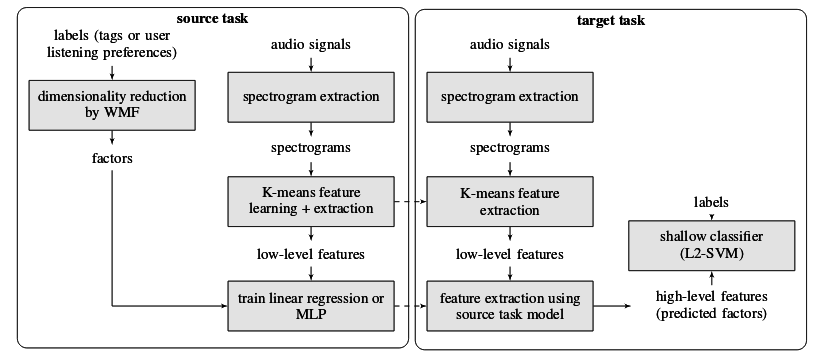
\includegraphics[width=0.95\textwidth]{specLeak1}
\caption{Schematic overview of the workflow of transfer learning\cite{TransferLearning}}
 \label{fig:transfer learning}
 \end{figure}
\FloatBarrier
\bigskip

\noindent \textbf{Source task}: 
The low-level features from audio spectrograms are learned through unsupervised learning by spherical K-Means. A multi layer perceptron is then stacked to obtain final prediction. So the output from the penultimate layer of MLP are treated as transferable features. To tackle problems created by redundant and sparse labels, dimensionality reduction is done in the label space using PCA. The model is then trained to predict the reduced label representation.
\bigskip

\noindent \textbf{Target task}
Next,  the trained models are used to extract features from other datasets, which are then passed to train shallow classifiers for different but related target tasks. This workflow is visualized in figure \ref{fig:transfer learning}. Dashed arrows indicate transfer of the learned feature extractors from the source task to the target task.
\bigskip


\subsection{Convolutional Neural Networks}
\label{convolution}
It can be seen that deep signal processing structures can be realized by stacking multiple shallow architectures (ref. \ref{stacked}). As feature learning was proving to be more efficient than hand crafted features, stacking learnable layers over one another became a hot area of research.  The idea was to replace the application specific dimension reductions with hierarchy of learnable convolution filters. 
\bigskip

\noindent \textbf{End-to-end learning for music audio. 2014\cite{EndToEnd}:}\\
\\
\noindent As shown in chapter 2, all operations including FFT can be defined in terms of convolutions. In this research they investigate whether it is possible to apply feature learning directly to raw audio signal. The signal was convolved with 3 layers of 1D convolutions followed by two fully connected layers. Thus, the feature and the classifier was trained in a single pipeline and this is called\textit{ end to end learning}. They compared the \textit{end to end learning} approach with convolutions from mel-spectrogram on MTT dataset (i.e, retaining STFT). Their algorithm is described below. Function $f$ is an element-wise logarithmic compression. It was found that, discarding STFT hurt the performance. CNN from mel-spectrogram achieved \textbf{AUC 0.8815}, but on including convolutions on audio signal AUC dropped to 0.8487.     
 
\begin{minipage}[t]{7.5cm}
  \vspace{0pt}  
  \begin{algorithm}[H]
    \caption{CNN(raw audio) [\textbf{0.84}]}
    \begin{algorithmic}[1]
      \Statex \textbf{Input :} $\textbf{a} \in \mathbb{R}^{N}$
      \Statex \textbf{Output :} $Pred \in \mathbb{R}^{L}$ 
      \State $\textbf{C}_{1}  = f(\textbf{a}\star\textbf{w}_{(256)}^{(256)})$
      \State $\textbf{C}_{2} =  MaxPool(ReLU(\textbf{C}_{1}\star\textbf{w}_{(32)}^{(1)}))$
       \State $\textbf{C}_{3} = MaxPool(ReLU(\textbf{C}_{2}\star\textbf{w}_{(32)}^{(1)}))$
       \State $\textbf{y} = FLATTEN(\textbf{C}_{3})$
       \State $Pred = \sigma(L(\textbf{W}_{2})ReLU(L(\textbf{W}_{1})\textbf{y}))$
   \end{algorithmic}
  \end{algorithm}
\end{minipage}%
\begin{minipage}[t]{7.5cm}
  \vspace{0pt}
  \begin{algorithm}[H]
    \caption{CNN(Mel-Spectrogram) [\textbf{0.88}]}
     \begin{algorithmic}[1]
      \Statex \textbf{Input :} $\textbf{a} \in \mathbb{R}^{N}$
      \Statex \textbf{Output :} $Pred \in \mathbb{R}^{L}$ 
      \State $\textbf{R}  = f(MEL(||STFT(\textbf{a})||^{2}))$
      \State $\textbf{C}_{1} =  MaxPool(ReLU(\textbf{R}\star\textbf{w}_{(32)}^{(1)}))$
       \State $\textbf{C}_{2} = MaxPool(ReLU(\textbf{C}_{1}\star\textbf{w}_{(32)}^{(1)}))$
       \State $\textbf{y} = FLATTEN(\textbf{C}_{2})$
       \State $Pred = \sigma(L(\textbf{W}_{2})ReLU(L(\textbf{W}_{1})\textbf{y}))$
   \end{algorithmic}
  \end{algorithm}
\end{minipage}
\FloatBarrier
\bigskip

\noindent \textbf{Experimenting with musically motivated convolutional neural networks. 2016\cite{MusicMotive}:}\\
\\
\noindent In the previous section, only 1D convolution with filter sizes directly motivated by hand-crafted methods were tested for comparison. But usually, the convolution operation allows flexibility in choosing the filter sizes. In this research, the authors discuss how convolution filters with different shapes can fit specific musical concepts. 
\begin{figure}[h]
       \begin{subfigure}[b]{0.3\textwidth}
        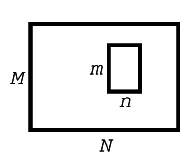
\includegraphics[width=\textwidth]{square}
        \caption{Rectangular filter }
        \label{fig:square}
       \end{subfigure}
	    \begin{subfigure}[b]{0.3\textwidth}
        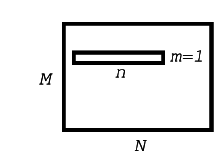
\includegraphics[width=\textwidth]{time}
        \caption{
        Time filter
        }
        \label{fig:time}
       \end{subfigure}
       	    \begin{subfigure}[b]{0.3\textwidth}
        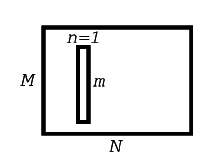
\includegraphics[width=\textwidth]{freq}
        \caption{
        Frequency filter
        }
        \label{fig:freq}
       \end{subfigure}
       \caption{Different Filter sizes}\label{fig:STFT}
\end{figure}
\FloatBarrier
\bigskip 
\noindent \textit{Time filters} can learn temporal cues (Onset, BPM and other rhythmic patterns), while \textit{frequency filters} can differentiate timbre and note. \textit{Rectangular filters} can learn short time sub-bands (Bass, kick, drums)\cite{MusicMotive}. However, because of hierarchical nature of deep networks, any filter should be theoretically capable of picking up the relevant cues. It was shown in their experiments that \textit{rectangular filters} or combination of time and frequency filters performed better than using just time / frequency filter. These experiments were however done for a genre classification task. 
\bigskip
 
\noindent \textbf{Automatic tagging using deep convolutional neural networks. 2016\cite{choi_cnn}:}\\
\\
\noindent Different CNN architectures were tested and the proposed model achieves close to state of art performance on MTT dataset (\textbf{0.894 AUC}). The audio samples were down-sampled to 12 KHz and convolutions were started from mel spectrogram (96 bins). They also compared MFCCs, convolutions over STFT and convolutions over Mel-log power spectrogram and report that the latter performs significantly better. 

    \begin{tabular}{ | p{5cm} | l |}
    \hline
    \textbf{Model} & \textbf{AUC} \\ \hline
    STFT $\rightarrow$ CNN &  0.846\\ \hline
    STFT $\rightarrow$ MEL $\rightarrow$ CNN &  \textbf{0.894}\\ \hline
    STFT $\rightarrow$ MEL $\rightarrow$ MFCC &  0.862 \\ \hline
    \hline
    \end{tabular}
    
\noindent Also, to exploit the advantage of PCA Whitening proven in \cite{MultiScale}\cite{featurelearn1}, Batch Normalization of frequency components is done. That is, data is centred to the batch mean and divided by batch variance. In Batch normalization however, the basis is not switched but the data is \textit{learned} to be scaled and shifted.
\begin{algorithm}
  \caption{$\textbf{\^{X}}$ = BATCHNORM($\textbf{X}$) }\label{Batch norm}
  \begin{algorithmic}[1]
    \Statex \textbf{Input :} $\textbf{X} \in \mathbb{R}^{B \times S \times Q}$, \Comment{$B$ is batch size}
    \Statex \textbf{Output :} $\textbf{\^X} \in \mathbb{R}^{B \times S \times Q}$ 
    \Statex \textbf{Parameters to learn :} $\gamma$ (Scale), $\beta$ (Shift) 
    \State $\bm{\mu}, \bm{\sigma}^{2} = FREQUENCY\_MEAN\_VARIANCE(\textbf{X})$ \Comment{$\bm{\mu},\bm{\sigma}^{2} \in \mathbb{R}^{S}$}
    \For{$i \in \{1,..,B\}$}
     \For{$j \in \{1,..,Q\}$}
       \State $\textbf{X}[i,:,j] \leftarrow \frac{\textbf{X}[i,:,j] - \bm{\mu}}{\sqrt{\bm{\sigma}}^{2} - \epsilon}$
      \EndFor
     \EndFor
     \State $\textbf{\^X} = \gamma\textbf{X} + \beta$
  \end{algorithmic}
\end{algorithm}
\FloatBarrier

\noindent The five layer proposed CNN architecture is shown below. The filters $\textbf{W}$ in each layer are the weights that will be learned. $Spatial\_Bn$ is similar to the normalization algorithm mentioned above, except that the normalization is done along the 1st axis of tensors $\textbf{C}$. $MaxPool_{i,j}$ is a dimensionality reduction done by pooling $(i,j)$ elements along $S$ and $Q$ directions respectively. $Elu$ is an element-wise non-linearity operation described in section \ref{training} 

\begin{algorithm}
  \caption{$\textbf{y}$ = $CHOI\_CNN(\textbf{R})$ }
  \label{alg:choicnn}      
  \begin{algorithmic}[1]
   \Statex \textbf{Input :} $\textbf{R} \in \mathbb{R}^{1 \times 96 \times 1366}$
   \Statex \textbf{Output :} $\textbf{y} \in \mathbb{R}^{1024}$ 
   \State $\textbf{R}_{n} = BatchNorm(\textbf{R})$
   \State $\textbf{C}_{1} = \textbf{R}_{n}\star\textbf{W1}_{(32)}^{(1,1)}$ \Comment{$\textbf{W1} \in \mathbb{R}^{32 \times 3 \times 3}, \textbf{C}_{1} \in \mathbb{R}^{32 \times S1 \times Q1}$}
   \State $\textbf{C}_{1} \leftarrow MaxPool_{(2,4)}(Elu(Spatial\_Bn(\textbf{C}_{1})))$ \Comment{$\textbf{C}_{1} \in \mathbb{R}^{32 \times T1 \times W1}$}
      \State $\textbf{C}_{2} = \textbf{C}_{1}\star\textbf{W2}_{(128)}^{(1,1)}$ \Comment{$\textbf{W2} \in \mathbb{R}^{128 \times 3 \times 3}, \textbf{C}_{2} \in \mathbb{R}^{128 \times S2 \times Q2}$}
   \State $\textbf{C}_{2} \leftarrow MaxPool_{(2,4)}(Elu(Spatial\_Bn(\textbf{C}_{2})))$ \Comment{$\textbf{C}_{2} \in \mathbb{R}^{128 \times T2 \times W2}$}
         \State $\textbf{C}_{3} = \textbf{C}_{2}\star\textbf{W3}_{(128)}^{(1,1)}$ \Comment{$\textbf{W3} \in \mathbb{R}^{128 \times 3 \times 3}, \textbf{C}_{3} \in \mathbb{R}^{128 \times S3 \times Q3}$}
   \State $\textbf{C}_{3} \leftarrow MaxPool_{(2,4)}(Elu(Spatial\_Bn(\textbf{C}_{3})))$ \Comment{$\textbf{C}_{3} \in \mathbb{R}^{128 \times T3 \times W3}$}
         \State $\textbf{C}_{4} = \textbf{C}_{3}\star\textbf{W4}_{(192)}^{(1,1)}$ \Comment{$\textbf{W4} \in \mathbb{R}^{192 \times 3 \times 3}, \textbf{C}_{4} \in \mathbb{R}^{192 \times S4 \times Q4}$}
   \State $\textbf{C}_{4} \leftarrow MaxPool_{(2,4)}(Elu(Spatial\_Bn(\textbf{C}_{4})))$ \Comment{$\textbf{C}_{4} \in \mathbb{R}^{192 \times T4 \times W4}$}
         \State $\textbf{C}_{5} = \textbf{C}_{4}\star\textbf{W5}_{(256)}^{(1,1)}$ \Comment{$\textbf{W5} \in \mathbb{R}^{256 \times 3 \times 3}, \textbf{C}_{5} \in \mathbb{R}^{256 \times S5 \times Q5}$}
   \State $\textbf{C}_{5} \leftarrow Elu(Spatial\_Bn(\textbf{C}_{5}))$ 
   \State $\textbf{y} = Flatten(\textbf{C}_{5})$ \Comment{$\textbf{y} \in \mathbb{R}^{1024}$}
  \end{algorithmic}
\end{algorithm}
\FloatBarrier

\noindent The features from convolutions then pass through a fully connected layer of size equalling  number of tags. The authors have then trained this model on MSD dataset and made the weights publicly available.

\section{Model Selection}
\label{model}
In section \ref{literature}, it was stated that when the feature is well \textit{organized} and encodes the \textit{variance} in the data, it becomes easier to attach a semantic meaning. Feature learning can increase robustness, but to learn an organized representation is not guaranteed. That is to say, the extracted feature should encode the information about it's discriminants  related to the task. Our brain differentiates sounds with energy changes, and this is approximated by MFCCs or Principal components (ref \ref{basis}) through proportionate energy variance from a mel-spaced spectrogram (ref \ref{mel}). But in section \ref{discriminants}, it was argued that the difference between music and speech is that, a music signal is composed of several superimposed \textit{rhythmic traces}. It was not clear if the classifier could decompose the rhythms from engineered features and hence there was this movement from feature engineering to feature learning. The results from the work [], where fully unsupervised technique is adopted for feature learning, shows that hand-crafted features does lose some information necessary for classification. But even the learned features were extracted from mel-spaced frequency spectrogram that does not exploit the harmonic encodings. That is, we still do not know if the learning algorithms extract the rhythms, thereby questioning the optimality of \textit{feature organization} (i.e, would the features learned for one task be optimal for auxiliary but related task?). However in general, it could be seen that feature learning performs better than MFCCs for multi-label classification task [auto tag, temporal].   
\bigskip

\noindent Music tagging problem is further complicated by the complexity of semantic assignments that reflect user preference. To get the right discriminants, the training method should be properly defined in the first place. In section \ref{problems}, the problems with content based methods that stem from training assumptions were pointed out. One of which was the social-factor assumption resulting from training on large datasets. This leaves us with the question, if the models trained by supervised learning on larger datasets [auto tagging, 1D] can be used for smaller datasets with different label-context. Secondly, the psychoacoustic assumptions resulting by training on short excerpts of music rather than whole song cause  vagueness. This is because, the currently available large datasets only contain short clips and the current algorithms generalize the tags for the whole song by merging tags from short sections of the song. Therefore, methods that hold better feature organization for songs of arbitrary length are also explored.   

\subsection{Transfer learning Vs MFCC}
\label{transfer}
To check if models trained on large datasets can be exploited for smaller datasets, \textit{transfer learning} from the model which achieves state of art performance with CNN [auto tagging] is compared with MFCC features. (It makes perfect sense to compare the state of art unsupervised feature learning algorithm [] as well, but in this thesis I stick to analysing CNNs). This will also show if features learned (stacked convolutions - ref. \ref{stacked}) through supervised training on large dataset attain better \textit{feature organization} than MFCCs. It is important to note that, better \textit{feature organization} simply does not mean that classifier identifies the \textit{rhythmic traces}.

\subsection{K-Means vs RNN}
\label{kmeans}
To summarize tags for songs of arbitrary length, most of the current algorithms classify short sections of the spectrogram separately and finally merge tags across different sections [end to end]. It is also possible to stack a \textit{decision tree} above the feature extractor to improve the performance, but that would not tell anything about the optimality of \textit{feature organization}. Hence for temporal pooling, only methods that directly work on content information are considered. Algorithm in [multi scale] is designed to handle songs of arbitrary length and it was seen that bag of words features trained using K-Means algorithm (see \ref{clustering}) proved efficient while testing on 29.1s excerpts from MTT dataset. However, it is not clear if these features are optimal choice for identifying rhythms.  It is also not known if the efficiency of K-Means will be retrained when tested on songs longer than 30s. Hence, this algorithm is compared with temporal summazization using Recurrent Neural Network (see \ref{rnn}). Supervised training with RNN might force the classifier to look for rhythmic content.    
        
 
 